\chapter[Resultados Parcias ]{Resultados Parciais}

\section{Resultados obtidos em MATLAB}
Em 2010 fabien lotte publicou um trabalho, demosntrando a classificação de sinais de EEG com LDA \cite{F.Lotte},usando o extrator de características \textit{common spatial pattenrs}(CSP) e outras
variações deste algoritmo. A base de dados usada foi a base do BCI \textit{competition} III, com os \textit{datasets BCI\_III\_DSIVa, BCI\_III\_DSIIIa e BCI\_IV\_DSIIa}. 

As implementações foram codificadas em \textit{Matlab}, e o autor chegou aos seguintes resultados mostrados na tabela \ref{resultlotte}.

\begin{table}[h]
\centering
\caption{Acurácias das classificações em \% usando o extrator CSP e classificador LDA, obtidas por \cite{F.Lotte}.}
\label{resultlotte}
\begin{tabular}{|l|l|l|l|l|l|}
\hline
\multicolumn{6}{|c|}{\textit{BCI III -  data set IVa}}  \\ \hline
Sujeito & A1    & A2    & A3    & A4    & A5   \\ \hline
CSP     & 66.07 & 96.43 & 47.45 & 71.88 & 49.6 \\ \hline
\end{tabular}
\end{table}
 
Reproduzir os resultados de \cite{F.Lotte}, é de suma importância para este trabalho, tanto para comparação quanto para o entendimento do algoritmo. 

Para executar o classificador já implementado por \cite{F.Lotte}, usou-se um laptop \textit{DELL}, equipado com processador \textit{Intel Core I5-4210U} CPU 2.4 GHz, 8 GB RAM e sistema operacional \textit{Windows 10},  ultilizando a base de dados \textit{BCI III -  data set IVa}, obteve-se os resultados contidos na Figura \ref{resultadoLotte}.

\begin{figure}[h]
	\centering
	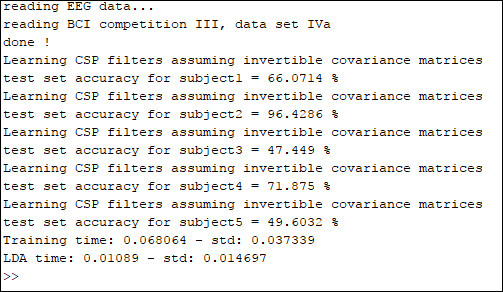
\includegraphics[keepaspectratio=true,scale=0.9]{figuras/resultados_csp_lda.png}
	\caption{Resultados obtidos  com CSP-LDA}
	\label{resultadoLotte}
\end{figure}

Observando os dados contidos na figura \ref{resultadoLotte}, pode ser analisar que a reprodução do algoritmo não necessitou de um alto tempo de execução, sendo o tempo médio de classificação de 0.01089 e desvio padrão de 0.014697 segundos.